\documentclass[12pt]{article}
\usepackage{fullpage}
\usepackage{epic}
\usepackage{eepic}
\usepackage{epsfig}

% \input{code}

% \pagestyle{empty}

% \setlength{\oddsidemargin}{0in}
% \setlength{\topmargin}{0.0in}
% \setlength{\textwidth}{6.5in}
% \setlength{\textwidth}{6.8in}
% \setlength{\textheight}{9.2in}

%\setlength{\oddsidemargin}{0in}
%\setlength{\topmargin}{-0.8in}
%\setlength{\textwidth}{6.8in}
%\setlength{\textheight}{9.5in}

\def\eps{{\varepsilon}}

\newcommand{\Mod}[2]{
{#1} ~ {\rm mod} ~ {#2}
}

\def\Prf{{\rm Pr}}


\newcommand{\Prb}[1]{
\Prf\left[{#1}\right]
}

\newcommand{\Prg}[2]{
\Prf\left[{#1}~|~{#2}\right]
}

\newcommand{\Exp}[1]{
E\left[{#1}\right]
}

\newcommand{\Expg}[2]{
E\left[{#1}~|~{#2}\right]
}



\begin{document}


\setlength{\fboxrule}{.5mm}\setlength{\fboxsep}{1.2mm}
\newlength{\boxlength}\setlength{\boxlength}{\textwidth}
\addtolength{\boxlength}{-4mm}
\begin{center}\framebox{\parbox{\boxlength}{\bf
The Structure of Information Networks \hfill Homework 2\\
CS/INFO 6850 Fall 2024 \hfill Due 6pm, Wednesday, October 2, 2024}}\end{center}
\vspace{5mm}

\def\ind{\hspace*{0.3in}}
\def\gap{\vskip 0.2in}
\def\rs{\vspace*{-0.0in}}
%\def\A{{\cal A}}
%\def\D{{\cal D}}
\newcommand{\Xomit}[1]{}
\newcommand{\cel}[1]{ {\lceil {#1} \rceil} }

\newcommand{\xhdr}[1]{\paragraph{{#1}.}}

\def\scenebreak{{\gap \center{\rule[.1in]{4.0in}{.01in}} \gap}}

Please hand in a single PDF file with all of the solutions,
and include your name and NetID in the file.

\medskip

For the style of analysis in the questions here,
you may find it helpful to review some of the arguments in the 
{\em Notes on Random Graphs and Expansion},
linked from the course home page at
https://www.cs.cornell.edu/courses/cs6850/2024fa/random-expander.pdf .
The questions below don't directly use the facts from these notes,
but many of the calculations use closely related reasoning.

\scenebreak

{\bf (1)} Consider a long, straight road, which we model
as a line segment of length $n$.
We drop a set of $k$ sensors randomly on this road ---
so each lands in a location selected uniformly and
independently from the interval $[0,n]$.

Now, each sensor has a transmitting range of $2$, so
it can communicate with any other sensor within a distance $2$ of it.
This mean that the random placement of the sensors
defines a random $k$-node graph $G$, in which the nodes are the sensors,
and we connect two by an edge if they can communicate with each other.
We'd like to choose $k$ large enough so that $G$ is
connected with high probability, and we can do this by reasoning as follows.

\gap
{\bf (a)} For an integer $j$ from $1, 2, \ldots, n$, let $E_j$
denote the event that no sensor lands in the interval $[j-1,j]$.
Give a formula for $\Prb{E_{j}}$ in terms of $n$ and $k$, together
with a brief explanation.

\gap
{\bf (b)} Argue that if none of the events
$E_j$ occurs, then the random graph $G$ defined above is connected.

\gap
{\bf (c)} Show using the Union Bound
that if we drop $k = 2 n \ln n$ sensors at random,
then with high probability the graph $G$ will be connected.
(In particular, with probability converging to $1$ as $n \rightarrow \infty$.)


\scenebreak

{\bf (2)}
A number of peer-to-peer systems on the Internet
are based on {\em overlay networks}:
rather than using the physical Internet topology
as the network on which to perform computation,
these systems run protocols by which nodes choose
collections of virtual ``neighbors'' so as to
define a higher-level graph 
whose structure may bear little or no relation to
the underlying physical network.

Many of these networks grow through the arrival of new participants,
who join by linking into the existing structure, and
this growth process has an intrinsic effect on the characteristics
of the overall network.

Here's a simple model of network growth, for which 
we can begin to analyze some structural consequences.
The system begins with a single node $v_1$.
Nodes then join one at a time; as each node joins, it executes
in a protocol whereby it forms a directed link to a single other node
chosen uniformly at random from those already in the system.
More concretely, if the system already contains nodes
$v_1, v_2, \ldots, v_{k-1}$ and node $v_k$ wishes to join,
it randomly selects one of $v_1, v_2, \ldots, v_{k-1}$
and links to this node.

Suppose we run this process until we have a system
consisting of nodes $v_1, v_2, \ldots, v_n$;
the random process described above will produce
a directed network in which each
node other than $v_1$ has exactly one out-going edge.
On the other hand, a node may have multiple
in-coming links, or none at all.
The in-coming links to a node $v_j$
reflect all the other nodes whose access into
the system is via $v_j$; so if $v_j$ has many
in-coming links, this can place a large load on it.
To keep the system load-balanced, then, we'd like all nodes to have a
roughly comparable number of in-coming links,
% Ideally, in building a system like this, we'd like
% the load to be distributed roughly uniformly across
% all participating nodes,
but that's unlikely to happen here,
since nodes that join earlier in the process are likely to have
more in-coming links than nodes that join later.
Let's try to quantify this imbalance as follows.
% across the nodes in the system.


\gap
{\bf (a)} 
Let $Z_j$ be a random variable corresponding to the in-degree of node $v_j$
(i.e., the number of in-coming links to node $v_j$).
Describe a way of writing $Z_j$ as a sum of random variables 
that each take the value $0$ or $1$.

\gap

{\bf (b)}
Applying linearity of expectation to your expression in (a), 
give a formula for the expected in-degree of node $v_j$
as a function of $n$ and $j$.
In particular, express your formula as the difference of
two harmonic numbers, $H_a - H_b$ for choices of $a$ and $b$
that you should find
(in terms of the parameters $n$ and $j$ in the model).
Recall that the harmonic numbers are defined as 
$$H_k = \sum_{j=1}^k \frac{1}{j}.$$
Provide a justification for your answer.

\gap

{\bf (c)}
Continuing with this model,
here's another way to look at the imbalances in the load on different nodes.
Let $X_j$ be a random variable equal to $1$ if node $v_j$ has
no incoming links, and equal to $0$ otherwise.
What is the expected value of $X_j$?
Provide a justification for your answer.

\gap

{\bf (d)}
Building on your answer to (c), and again using 
linearity of expectation, 
give a formula for the expected number of nodes
with no incoming links
in a network grown randomly according to this model.
Try to write your formula if possible in ``closed form'' --- that is, written
without any lengthy summations or $\sum$ notation.
Provide a justification for your answer.

\begin{figure*}[t]
\begin{center}
\hspace*{0.1in} 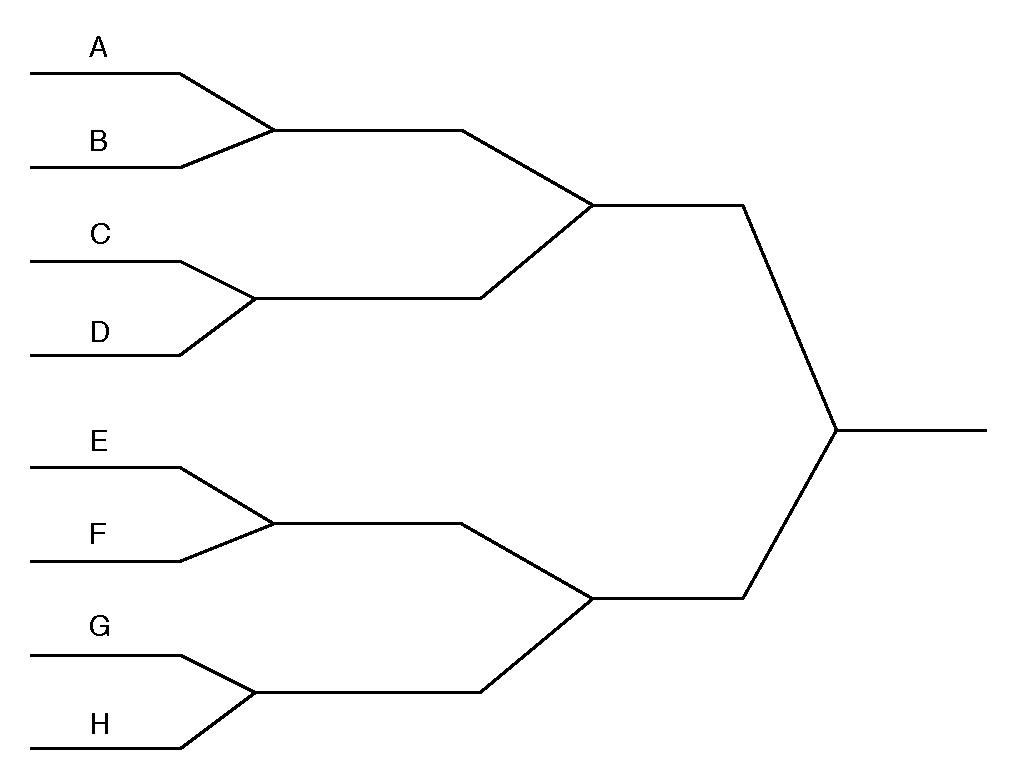
\psfig{figure=elim-blank,width=4.0in}\caption{An 
elimination tournament of the kind described in Question 3,
with just the initial contestants, before any matches have been played.
\rs
\label{fig:elim-blank}
}
\end{center}
\end{figure*}

\begin{figure*}[t]
\begin{center}
\hspace*{0.1in} 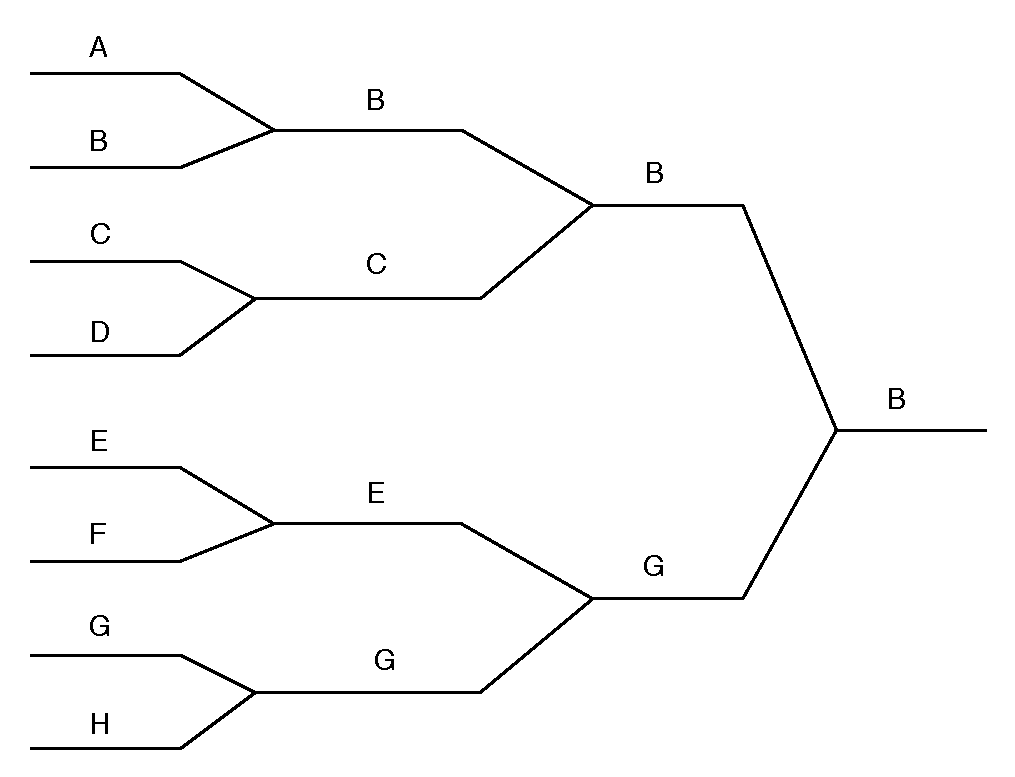
\psfig{figure=elim-filled,width=4.0in}\caption{The 
results of the elimination tournament from Figure \ref{fig:elim-blank}, after all matches have been played.
\rs
\label{fig:elim}
}
\end{center}
\end{figure*}

\scenebreak

{\bf (3)} 
Consider a standard $k$-round, single-elimination tournament,
such as you see in championship competitions for a number of different sports.
Specifically, $n = 2^k$ contestants start out at the beginning,
and in each round the current contestants play each other in specified pairs,
with the winners moving on to the next round.
An example with $k = 3$ and $2^3 = 8$ initial contestants
is depicted in Figures~\ref{fig:elim-blank} and \ref{fig:elim}.
One can also picture this as a complete binary tree with
the initial contestants at the leaves, and each internal node
corresponding to a match-up of two surviving contestants.

Suppose that a group of people get together to bet on the results
of the tournament, predicting the outcome of each match.
If you're taking part in this group, you get
a copy of a blank table with
just the initial contestants filled in
(as in Figure~\ref{fig:elim-blank}),
and you're asked to fill in all the entries for the subsequent rounds.
Crucially, all entries must be filled in before 
any matches are played.
The filling-in should be consistent, in that if you
write a person's name as a winner in round $j$,
you should also have guessed that they're a winner 
in the previous round $j-1$.

Let's consider how well we'd expect someone to do 
at guessing these results, if they had no information about
any of the contestants and were just guessing at random.
We'll model this lack of information by assuming that
after they fill in their table, 
each match's outcome is 
determined by an independent fair coin flip.  (So each contestant
is equally likely to win and advance to the next round,
where their fate will be determined by the next coin flip).

Let $p(j)$ denote the probability that at least one of 
a person's guesses for the entries in
round $j$ turn out to be correct.
That is, we look at all their guesses for the contestants
in round $j$, and see if any of these contestants 
actually made it to round $j$.

\gap

{\bf (a)}
Write an expression for $p(j)$ as a function of $j$ and $n$.
Provide a justification for your answer.

\gap
\gap

{\bf (b)}
Is there a constant value $\alpha^*$ that is {\em critical} for
this probability 
in the following sense?
\begin{quote}
{\em If $\alpha < \alpha^*$ then 
$$\lim_{n \rightarrow \infty} p(\alpha \log n) = 1,$$
while if 
$\alpha > \alpha^*$ then 
$$\lim_{n \rightarrow \infty} p(\alpha \log n) = 0.$$}
\end{quote}
(Recall that $k = \log n$; all logarithms here are base $2$.)
In your answer, either specify such a value of $\alpha^*$ and
justify why it is critical, or argue why there is no
critical value of $\alpha^*$.
% {\em (Note: in your answer, you can use the fact that for
% any constants $c > 0$ and $\eps > 0$, it is the case that
% $\lim_{n \rightarrow \infty} n^c e^{- n^{\eps}} = 0$.)}

% \scenebreak


\end{document}

